\documentclass[10pt]{beamer}

\usepackage{mdframed}
\usepackage{minted}
\definecolor{bg}{rgb}{0.90,0.30,0.30}
\BeforeBeginEnvironment{minted}{\begin{mdframed}[backgroundcolor=black!10]}
\AfterEndEnvironment{minted}{\end{mdframed}}

\usetheme[progressbar=frametitle]{metropolis}
\usepackage{appendixnumberbeamer}

\usepackage{graphicx}

\usepackage{booktabs}
\usepackage[scale=2]{ccicons}

\usepackage{pgfplots}
\usepgfplotslibrary{dateplot}

\usepackage{xspace}
\newcommand{\themename}{\textbf{\textsc{metropolis}}\xspace}

\title{Haskell \& Servant}
\subtitle{An introduction to the Functionnal Programming paradigm}
\date{\today}
\author{FlogFR}
\institute{
\begin{center}

\includegraphics[height=3cm]{Chapeau-Pipe.png}
\end{center}
}

\begin{document}

\maketitle

\section{Only my opinion in this talk, trust me}

\begin{frame}{My vision of computer science}
\begin{itemize}
\item Software is data, and calculation on data (and displaying the results)
\item Software is for all kind of industry
\item Software development should be as easy/difficult as the problem
\end{itemize}
\end{frame}

\begin{frame}{My experience}
\begin{itemize}
\item First love with C++
\item Perl as the first language profesionnaly
\item Years of experience in Python
\item Years of experience in PostgreSQL
\item Now full-time Sysadmin/SRE: Good knowledge of what is a production environment
\item Never really finished any side project I started. (but I have 1000+ POCs somewhere in the cloud)
\end{itemize}
\end{frame}

\begin{frame}{My feelings}
\begin{itemize}
\item The style of coding in all the language I used is not consistent across projects
\item Refactoring/Updating the architecture of a medium to big size project (200k+ LOC) is a pain in Python. Mostly because you touch something in one tiny place, and it breaks something at the other side of world.
\item The object paradigm is obfuscating the calculation in the code
\item I miss having a compiler (like the one for C++)
\item Hard to understand the representation of the data in memory in Python
\end{itemize}
\end{frame}

\section{The solution to all your problems}

\begin{frame}{Solution}
\begin{itemize}
\item Seriously? You thought there's a universal solution to all your problem?
\end{itemize}
\end{frame}

\section{I have a web project}

\begin{frame}{My requirements}
\begin{itemize}
\item Minimalist architecture and infrastructure to iterate quickly
\item No brainer: PostgreSQL + Sqitch
\item Give a try to what I heard is "FP"
\end{itemize}
\end{frame}

\begin{frame}{Let's test ELM}
\begin{itemize}
\item https://elm-lang.org/
\item Let's do the official guide (https://guide.elm-lang.org/)
\item Let's create some proof of concept with ELM (ended up to be almost a copy of the SPA example https://github.com/rtfeldman/elm-spa-example)
\end{itemize}
\end{frame}

\begin{frame}{What I learned from ELM}
\begin{itemize}
\item pro: Amazing centralized documentation: https://package.elm-lang.org/
\item pro: My POC was production ready from day 1 (mostly because of type safety, and the tooling is minimal/simple)
\item pro: Finished a small SPA project in ~2 months (learning the language included)
\item cons: I didn't learn how to unit test because of the transpiler + typing
\item cons: The roadmap is not clear of the language
\item cons: Frustrated by the language after a time (repetitive)
\end{itemize}
\end{frame}

\section{So I finished one project?}

\begin{frame}{So I finished one project?}
\begin{itemize}
\item Yes
\end{itemize}
\end{frame}

\begin{frame}{Let's analyze this success}
\begin{itemize}
\item I like the syntax of ELM (subset of haskell)
\item I Love the transpiler
\item I Love the strong typing
\end{itemize}
\end{frame}

\section{Can I apply now this success to the backend development?}

\begin{frame}{Now Haskell}
\begin{itemize}
\item Created in ~1990, financed by Microsoft (~20 years of reseach on the language/compiler)
\item *Pure* Functional Programing
\item Compiled (marvelous compiler, a masterpiece)
\item Lazy (default performance comparable to C programs - be careful of the benchmark online about Rust etc. We had the same with Go couple of years ago)
\item Strongly typed - Value level, and the Type level
\item Mature and friendly community, stable eco-system…
\item Close to mathematics
\end{itemize}
\end{frame}

\section{What else? Let's start to learn it!}

\begin{frame}{Learning Haskell}
\begin{itemize}
\item Books
\item Haskell Wiki
\item Community (IRC, Github)
\item Github Searches
\item Project! Project! Project!
\end{itemize}
\end{frame}

\begin{frame}{The amazing Haskell}
\begin{itemize}
\item Haskell documentation search engine "hoogle"
\end{itemize}
\end{frame}

\begin{frame}[fragile]{The amazing Haskell} 
\begin{itemize}
\item Hoogle documentation
\end{itemize}
\begin{minted}[
  fontsize=\footnotesize
]{haskell}
-- Search: Maybe a -> Bool
-- Results:
isJust :: Maybe a -> Bool
\end{minted}
\end{frame} 

\begin{frame}{The amazing Haskell}
\begin{itemize}
\item Haskell documentation search engine "hoogle"
\item Code makes it straightforward to see the representation of the data and the calculation
\end{itemize}
\end{frame}

\begin{frame}[fragile]{The amazing Haskell} 
\begin{minted}[
  fontsize=\footnotesize
]{haskell}
\end{minted}
\end{frame} 

\begin{frame}{The amazing Haskell}
\begin{itemize}
\item Haskell documentation search engine "hoogle"
\item Code makes it straightforward to see the representation of the data and the calculation
\item Lazyness = performant code by default
\end{itemize}
\end{frame}

\begin{frame}[fragile]{The amazing Haskell} 
\begin{minted}[
  fontsize=\footnotesize
]{haskell}
-- recursive thinking with performance
\end{minted}
\end{frame} 

\begin{frame}{The amazing Haskell}
\begin{itemize}
\item Haskell documentation search engine "hoogle"
\item Code makes it straightforward to see the representation of the data and the calculation
\item Lazyness = performant code by default
\item Easy composition of code (thanks to typeclass)
\end{itemize}
\end{frame}

\begin{frame}[fragile]{The amazing Haskell} 
\begin{itemize}
\item Generic algorithm
\end{itemize}
\begin{minted}[
  fontsize=\footnotesize
]{haskell}
class SqlRow a where
  fromSqlResultRows :: Result -> IO [a]
  fromSqlResultRows sqlResult = do
    (Row nbRows) <- ntuples sqlResult
    let rows = [0..(nbRows-1)]
    mapConcurrently (\k -> fromSqlResultRow sqlResult k) rows
\end{minted}
\end{frame} 

\begin{frame}{The amazing Haskell}
\begin{itemize}
\item Haskell documentation search engine "hoogle"
\item Code makes it straightforward to see the representation of the data and the calculation
\item Lazyness = performant code by default
\item Easy composition of code (thanks to typeclass)
\item Monad (context of calculation) limiting the side effects
\end{itemize}
\end{frame}

\begin{frame}[fragile]{The amazing Haskell} 
\begin{itemize}
\item Controlling the side effects
\end{itemize}
\begin{minted}[
  fontsize=\footnotesize
]{haskell}
-- example 1 (Monad)
type HandlerM = ReaderT SharedEnv (LoggingT Handler)
-- userLoggedInOrRedirect :: Session -> HandlerM ()

-- example 2 (TypeClass)
foldr :: Foldable t => (a -> b -> b) -> b -> t a -> b
\end{minted}
\end{frame} 

\begin{frame}{The amazing Haskell}
\begin{itemize}
\item Haskell documentation search engine "hoogle"
\item Code makes it straightforward to see the representation of the data and the calculation
\item Lazyness = performant code by default
\item Easy composition of code (thanks to typeclass)
\item Monad (context of calculation) limiting the side effects
\item Learning curve and possibilities unlimited (related also to monad)
\end{itemize}
\end{frame}

\begin{frame}[fragile]{The amazing Haskell} 
\begin{itemize}
\item Monad/Context of calcultation is also a way of thinking
\item Thus you can specialize in any industry
\end{itemize}
\begin{center}
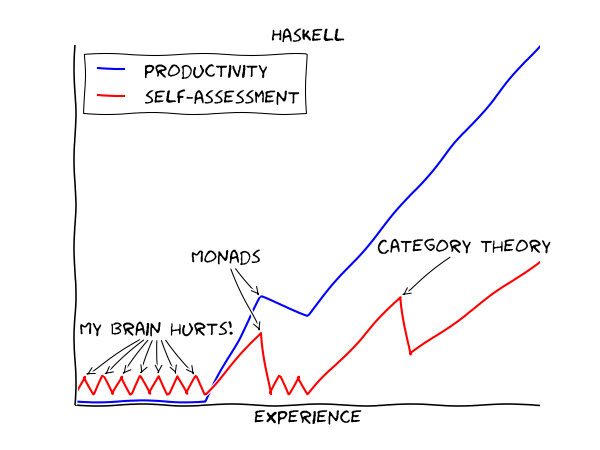
\includegraphics[height=6cm]{monad-haskell-learning-curves.png}
\end{center}
\end{frame} 

\begin{frame}{The amazing Haskell}
\begin{itemize}
\item Haskell documentation search engine "hoogle"
\item Code makes it straightforward to see the representation of the data and the calculation
\item Lazyness = performant code by default
\item Easy composition of code (thanks to typeclass)
\item Monad (context of calculation) limiting the side effects
\item Learning curve and possibilities unlimited (related also to monad)
\item Easy maintainability and refactoring of code (thank you compiler + strongly type + monad)
\end{itemize}
\end{frame}

\begin{frame}[fragile]{The amazing Haskell} 
\begin{minted}[
  fontsize=\footnotesize
]{haskell}
-- example 1 (Monad)
type HandlerM = ReaderT SharedEnv (LoggingT Handler)
-- userLoggedInOrRedirect :: Session -> HandlerM ()

-- example 2 (TypeClass)
foldr :: Foldable t => (a -> b -> b) -> b -> t a -> b
\end{minted}
\end{frame} 

\begin{frame}{The amazing Haskell}
\begin{itemize}
\item and I'm forgetting lots of others pros…
\item cons: I still didn't learn how to do unit tests in Haskell…
\end{itemize}
\end{frame}

\section{I want to make an API for my project, in Haskell!}

\begin{frame}{The amazing Servant}
\begin{itemize}
\item Set of Haskell library to create API
\item +1100 github stars
\item Describe an API at the Type Level
\item Structure re-usable by all libraries
\end{itemize}
\end{frame}

\begin{frame}{The amazing Servant}
\begin{itemize}
\item Describe an API at the Type Level
\end{itemize}
\end{frame}

\begin{frame}[fragile]{The amazing Servant} 
\begin{minted}[
  fontsize=\footnotesize
]{haskell}
type FrontAPI =
    -- Public Area
    Header "X-Real-IP" Text :> QueryParam "lat" Double :> ... :> Get '[HTML] H.Html
    -- ...
    :<|> "account" :> Get '[HTML] H.Html
    :<|> "account" :> MultipartForm Mem AccountForm :> Post '[HTML] H.Html
\end{minted}
\end{frame} 

\begin{frame}{The amazing Servant}
\begin{itemize}
\item Describe an API at the Type Level
\item Re-usable Type level API structure
\end{itemize}
\end{frame}

\begin{frame}[fragile]{The amazing Haskell} 
\begin{minted}[
  fontsize=\footnotesize
]{haskell}
-- Swagger in one line of code
BSL8.putStrLn $ encode $ toSwagger (Proxy :: Proxy UserAPI)
  & info.title        .~ "User API"
  & info.version      .~ "1.0"
  & info.description  ?~ "This is an API for the Users service"
  & info.license      ?~ "MIT"
  & host              ?~ "example.com"
:}
\end{minted}
\end{frame} 

\begin{frame}{The amazing Servant}
\begin{itemize}
\item Describe an API at the Type Level
\item Re-usable Type level API structure
\item Composition of API
\end{itemize}
\end{frame}

\begin{frame}[fragile]{The amazing Servant} 
\begin{minted}[fontsize=\footnotesize]{haskell}
type API =
  "static" :> Raw
  :<|> "blog" :> BlogAPI
  :<|> "login" :> ServerLoginAPI
  :<|> MonitoringAPI
  :<|> AuthProtect "custom-auth" :> FrontAPI
  :<|> AuthProtect "custom-auth" :> "api" :> "v1" :> APIV1
  :<|> AuthProtect "custom-auth" :> "admin" :> AdminAPI
\end{minted}
\end{frame} 

\begin{frame}{Contact}
  Florian Grignon - @FlogFR\newline
  Private Detective @Infratelier

  \begin{center}\url{https://github.com/FlogFR}\end{center}
  \begin{center}\url{grignon.florian@gmail.com}\end{center}
\end{frame}

\begin{frame}{Thank You}

  \begin{columns}[T,onlytextwidth]
    \column{1.00\textwidth}
    To my dear friend and associate:
      \begin{itemize}
        \item Dr Watson
      \end{itemize}
    A personnal thank you to:
      \begin{itemize}
        \item Organizers and sponsors of the events
        \item DBAs Colleagues @PeopleDoc
        \item PostgreSQL community
      \end{itemize}
  \end{columns}

\end{frame}

\appendix

\begin{frame}[fragile]{Questions}
  FlogFR - grignon.florian@gmail.com - https://github.com/FlogFR
  \begin{center}
  
\includegraphics[height=5cm]{Chapeau-Pipe.png}
  \end{center}
\end{frame}

\end{document}
